\chapter{Related works} \label{chap:survey}

\section{Recognition Application}
There has been numerous application that can do certain object detection. Google Lens is an AI-powered application, designed to bring up relevant information related to the object. For example, when pointing the camera at a puppy, the application will be able to detect it and give related information, such as breeds, approximate age and food type. It uses Region Proposal Network (RPN) to detect character box for OCR and Convolutional Neural Network (CNN) with a Long short-term memory (LSTM) to detect object in image. Released in December 2019, Microsoft Math Solver application can recognize letters, math characters and symbols using OCR, categorizing using a natural language processing algorithm and then solved step by step. There are also multiple candidates that can detect certain type of object such as Aipoly Vision, ScreenShop, Flow and Vivino.

\section{Object detection methods}
\subsection{Introduction}
Object detection is a critical task in computer vision field that deal with multiple types of a certain visual object such as animal, flower, people, diagram,... It acts as the fundamental of other tasks such as segmentation, object tracking, image captioning, event detection, scene understanding and activity recognition,... The goal of object detection is to give basic knowledge to the computer: ''What is this object?'' and if possible, return the coordinate where this object locates . The object detection task can be divided into two topics: ''general detection'' and ''specific detection''. The first topic indicates the ability to detect instances of an object under an uniform condition and thus simulate human eyes with automotive car as an example. The other topic covers the detection of object under specific scenarios such as face detection, voice detection, text recognition, diagram recognition, etc. Object detection is widely used in multiple applications, such as autonomous driving, robot and crime prevention.

\subsection{Traditional detector}
Most of the early object detection algorithms were built based on manual made features with multiple complex model. Due to the lack of resources and image size, a number of speed up methods are required.

In 2001, P. Viola and M. Jones achieved real-time face detection using sliding windows \cite{VJ1,VJ2}. The algorithm go through all possible locations and scales in an image to find the human face. It speeds up the computational process by involving three important techniques. The first one, integral image speeds up box filtering or convolution process using Haar wavelet as the feature representation of an image. The second one, feature selection using Adaboost algorithm to select a small set of features from a huge set of feature pools. The third one, A multi-stage detection paradigm reduces its computation by spending less time on background than on face possibility location. Although the algorithm is simple, it exceeds the current computational power of computer at that time. 

Histogram of Oriented Gradients (HOG) was created in 2005 by N.Dalal and B.Triggs \cite{HOG}. It is designed to be computed on a grid of equal cells and use overlapping local contrast normalization to improve accuracy. To detect object of different size, HOG resize the input image for multiple times to match with detection window size. It has been an important foundation of many object detectors and a large variety of computer vision applications.\cite{HOG1,HOG2}

\subsection{CNN-based Detector}
As the traditional methods showing their disadvantages by becoming more and more complex, the progress has been slow down, researchers tried to find an alternative to increase the accuracy and performance. In 2012, Krizhevsky et al. brought back the age of Convolutional Neural Network with a paper on classification with ImageNet \cite{16}. As a DCNN can classify the image based on feature set, subsequent papers show their interest in the newly found method in object detection. Over the past decades, multiple network models has been proposed and studied to improve the accuracy in detection such as LeNet-5 \cite{19}, AlexNet \cite{20}, VGG-16 \cite{21}, Inception \cite{22,23}, ResNet \cite{24},etc. Studies also discover techniques that improve the training process and prevent overfitting, for example, dropout \cite{20}, Auto Encoder \cite{25}, Restricted Boltzmann Machine (RBM) \cite{26}, Data Augmentation \cite{27} and Batch Normalization \cite{28}.

\begin{figure}[!t]
\centering
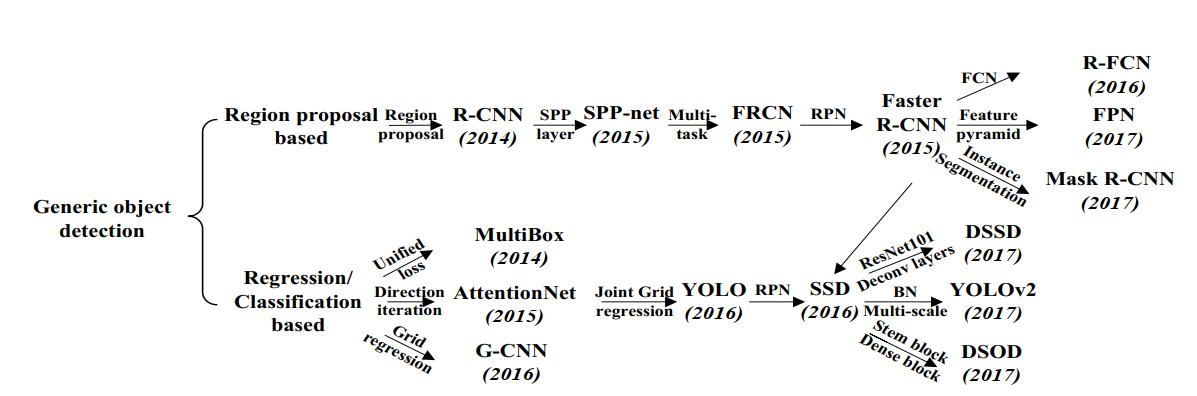
\includegraphics[width=14cm]{Images/recognition/Object_Detection.png}
\caption{Object detection}
\label{fig:object detection}
\end{figure}

There are two main groups in CNN-based detection: ''two stages detecion'' and ''one stage detection''. In the first group, firstly the image will be examined to generate proposals, and these proposals are delivered to another network for classification. In the second group, the object will be detected and classified directly within one network model.

\subsubsection{CNN-based Two Stages Detection (Regional Proposal based)}
Released in 2014 by Girshick et al.\cite{17,18}, R-CNN is the first attempt in building a Convolutional Neural Network for object detection. The idea of R-CNN is divided into three main stages:
\begin{itemize}
    \item Proposals are generated by selective search.
    \item Proposals are resized to fixed resolution. These proposals are then used in CNN model to extract the feature map.
    \item Feature map is classified using SVMs for multiple classes to provide the final bounding box.
\end{itemize}
Despite having certain advantages comparing with traditional methods and bringing CNN back to practical use, R-CNN has some fatal disadvantages. The training has multiple stages and feature maps are stored separately thus increase time and space complexity. Moreover, The number of overlapped proposals are really high (over 2000 proposals for an image). The CNN model also requires a fixed size image, so any input must be resized and in certain occasions the object may get cropped, creating unwanted distortion.
    
Later in the same year, He et al. introduced a novel CNN architecture named SPP-Net \cite{29} using Spatial Pyramid Matching (SPM) \cite{30,31}. The Convolutional Neuron Network is combined with a Spatial Pyramid Pooling (SPP) layer, make the network able to generate a fixed length feature representation without scaling the input image. The model removes the proposal overlapping and the need to resize image, however, it still require a multi-step training including feature extraction, network fine-tuning, SVM training and bounding box regressor. Additionally the convolution layers before the SPP cannot be modified with the algorithm shown in \cite{29}
    
In 2015, Girshick proposed Fast R-CNN \cite{32}, a model with ability to do multi-task on classification and bounding box regression within the same network. Similar to SPP-Net, the whole image is processed with convolution layers to produce feature maps. Then, a fixed-length feature vector is extracted from each region proposal with a region of interest (RoI) pooling layer. Each feature vector is then fed into a sequence of fully connected layers before branching into two output, one is then used for classifier and the other encodes the bounding box location. Regardless of region proposal generation, the training of all network layers can be processed in a single stage, saving the extra cost on storage. 
    
In the same year, Ren et al. introduced Faster R-CNN, a method to optimize Fast R-CNN further by altering the proposal generation using selective search by a similar network called the Region Proposal Network (RPN) \cite{33}. It is a fully-convolutional network which has the ability to predict object bounds and scores at each position as the same time. With the proposal of Faster R-CNN, region proposal based CNN architectures for object detection can be trained
in an end-to-end way. However, the alternate training algorithm is very time-consuming and RPN does not perform well when dealing with objects with extreme scales or shapes. As a result, multiple adjustments have been made. Some noticeable improvements are Region-based fully convolutional network (R-FCN) \cite{34}, Feature Pyramid Network (FPN) \cite{35}, and Mask R-CNN \cite{36}. We will look in the details of these methods in the next chapter.

\subsubsection{CNN-based One Stage Detection (Regression/Classification based)}
Region proposal based frameworks are composed of several correlated stages, including region proposal generation, feature extraction, classification and bounding box regression. Even in Faster R-CNN or its variant, training the parameters is still required between the Region Proposal Network and detection network. As a result, achieving real time detection with Two Stages Detection is a big challenge. One Stage Detection, on the other hand, deal with the image directly by mapping image pixel to bounding box coordinates and class probabilities. 

\begin{itemize}
    \item You Only Look Once (YOLO):
    YOLO \cite{37} was proposed by J.Redmon et al. in 2015 as the first entry to the One Stage Detection era. This network divides the image into regions and predicts bounding boxes and probabilities for each region simultaneously. The YOLO consists of 24 convolution layers and 2 FC layers, of which some convolution layers construct ensembles of inception modules with 1 × 1 reduction layers followed by 3 × 3 conv layers. Furthermore, YOLO produces fewer false positives on background, which makes the cooperation with Fast R-CNN become possible. An improved version, YOLO v2,v3 and v4 was later proposed in, which adopts several impressive strategies, such as BN, anchor boxes, dimension cluster and multi-scale training.\cite{38,39,40}.

    \item Single Shot MultiBox Detector (SSD):
    SSD \cite{41} was proposed by W. Liu et al. in 2016 as the second entry of the One Stage Detector. SSD introduces the multi-reference and multi resolution detection techniques which significantly improves the detection accuracy. The main difference between SSD and any other detectors is that SSD detects objects of many different scales on different layers of the network rather than detect at the final layer.
    
    \item RetinaNet:
    RetinaNet \cite{42} uses a Feature Pyramid Network(FPN) with a CNN-based Backbone. FPN involves adding top level feature maps with the feature maps below them before making predictions. It usually involves upscaling the top level map, dimensionality matching of the map below using a 1x1 Convolution and performing element wise addition of both. RetinaNet achieves comparable result to Two Stages Detection while keeping much higher speed. 
    
    \item Refinement Neural Network for Object Detection (RefineDet):
     RefineDet \cite{43} is based on a feed forward Convolutional Network that is similar to SSD, produces a fixed number of bounding boxes and the scores indicating the presence of different classes of objects in those boxes, followed by the non-maximum suppression to produce the final result. RefineDet is formed by two inter-connected modules:\\
     $\bullet \quad$ Anchor Refinement Module (ARM): Remove negative anchors and adjust the locations/sizes of anchors to provide initialization for the regressor.\\
     $\bullet \quad$ Object Detection Module (ORM): do regressing object locations and predict multi-class labels based on the refined anchors.\\
     There are three core components in RefineDet: Transfer Connection Block (TCB) converts the features fro ARM to ODM; Two-step Cascaded Regression does regressing the locations and sizes of objects; Negative Anchor Filtering will reject well-classified negative anchors and reduce the imbalance problem. Further information will be discussed in the next chapter.
\end{itemize}

\section{Diagram detection}
In general, diagram detection can be grouped into two smaller areas: Online Diagram Recognition and Offline Diagram Recognition. In online recognition, the model is usually a RNN to recognize each stroke and generate candidate matches.
Valois et al. \cite{44} proposed a method for recognizing electrical diagrams. Each set of ink strokes is detected as a match with corresponding confidence factor using probabilistic normalization functions. Its disadvantage is the simplicity of the system and their low accuracy, prevent it from being used in real situations. Feng et al. \cite{45} used a more modern technique in detecting electrical circuits. Symbol hypotheses generation and classification are generated using a Hidden Markov Model (HMM) and traced on 2D-DP. However, it has a drawback of complexity when the diagram and number of hypotheses is large, makes it impractical for real life cases. ChemInk \cite{46}, a system for detecting chemical formula sketches, categorizing strokes into elements and bonds between them. The final joint is performed using conditional random fields (CRF), which combines features from a three layers hierarchy: inkpoints, segments and candidate symbols. Qi et al \cite{47}. used a similar approach to recognize diagram structure with Bayesian CRF - ARD. These methods outperforms traditional technique, but the difficulty in joining the features using pairwise at the final recognition step make them harder for future adaptations. Coming to Flowchart recognition, after the release of the Online Handwritten Flowchart Dataset (OHFCD), multiple researches took place in resolving this dataset. Lemaitre et al \cite{48}. proposed DMOS (Description and MOdification of the Segmentation) for online flowchart recognition. Wang et al. \cite{49} used a max margin Markov Random Field to perform segmentation and recognition. In \cite{50} they extend their work by adding a grammatical description that combines the labeled isolated strokes while ensuring global consistence of the recognition. Bresler et al. proposed a pipeline model where they separate strokes and text by using a text/non-text classifier then detect symbol candidates using a max-sum model by a group of temporally and spatially close stroke. The author also propose an offline extension that uses a preprocessing model to reconstruct the strokes from flowchart \cite{51,52}.

While online flowchart recognition detects candidates based on stroke, offline flowchart recognition receives an image from the user and use it to generate the diagram. It might be possible to reconstruct online stroke from offline data \cite{53}, however, that preprocessing step might not be necessary because we can recognize the whole diagram structure independently with strokes. As online recognition seem to attract more researchers, there has not been many studies about offline detection. A. Bhattacharya et al. \cite{54} uses morphological and binary mapping to detect electrical circuit. Although it may work on a smaller scale, using binary mapping may not be able to detect curve or zig-zag lines. Julca-Aguilar and Hirata proposed a method using Faster R-CNN to detect candidates and evaluate its accuracy on OHFCD. The model is able to detect components in the diagram, including arrows, however, it is not able to detect the arrow head. 
\section{Handwriting character recognition techniques for English alphabets} 
Handwriting recognition is a study domain in fields of image processing and pattern recognition which is popular and complicated in the current day. It contributes immensely to the
sequence of a computerization technique and could enhance the interface among human and machine in so many purposes. This process primarily start with preprocessing procedure which is followed by line segmentation, normalization, feature extraction, recognition and transcriptions according to \cite{12}. The preprocessing includes the process that improves the structure of the image which is more suitable in segmentation. In the segmentation procedure, the raw image is segmented into single characters and after that, the procedure reconstruct each character in m x n pixels to the training network. Next is about feature extraction technique, which affects recognition percentage. There are numerous of feature extraction methods which are mentioned in the research of \cite{13}. Additionally, according to \cite{12}, the frequently used feature extraction techniques are Contour profiles, Deformable templates, Fourier descriptors, Gabor
features, Gradient feature, Graph description, Geometric moment invariants, Template matching, Unitary Image transforms, Projection Histograms, Zoning, Zernike Moments and Spline curve approximation.
\subsection{Preprocessing}
In preprocessing procedure, there are many actions needs to be executed, which are noise removing, binarization, edge detection, dilation and filling, processed image for feature extraction according to \cite{12}. In noise removing phase, the reason for this phase is that scanned documents can be contaminated with dust, dots, or lines, which are classified as noise that has a negative impact on the recognition results. Therefore, image is applied with smoothing and non linear operations to improve the image quality. In addition, for text line which is not horizontally align during scanning process, the skew correction can be applied on the document or line level. In the preprocessing procedure, skew correction is applied on the document level.
\subsection{Line segmentation}
In line segmentation, this phase separates the image whose structure in a sequence of alphabet characters into sub image which contains a single character by conveying a number to every alphabet utilizing a labeling procedure. This labelling provides knowledge about number of characters in the image. Every single character is restructured into 90*60 pixels for categorization and recognition stage.
\subsection{Normalization}
After line segmentation, normalization is performed to eliminate the differences that complicate the categorization and decrease the recognition percentage of the similar character or word across different writers. The most general basis of variability in handwritten alphabet images is incline and text volume according to \cite{12}. Slant correction techniques is applied to correct the inclination in the writing style. By applying a shear transformation, the writings slant is transformed into its upright position. A shear transformation is applied in many directions. For each direction, the transformed image data are added with pixel values of the same image that are vertically shifted by distance d and –d.
\subsection{Feature extraction}
In feature extraction step, there are two main approaches which are used holistic and analytic \cite{12}. In holistic recognition, each word is considered to a class and is recognized as whole word. On the other hand, the other approach is based on character segmentation-free recognition.
Based on \cite{12}, features used in holistic offline recognition systems are categorized into high,
middle, and low levels. The high level removes the features from the entire phrase image, the middle level removes features from the letters, and the low level removes features from the sub letters. There are various types of holistic features which are represents in \cite{12}.
In analytic recognition schemes, the image is representing as a chain of characteristics. This scheme uses a slicing window which is shifted from left to right. At each position n, a characteristic vector fn is calculated from just the pixel within the slicing window. Two major slicing window scheme characteristics are profile characteristics and window characteristics \cite{12}.
\subsection{Recognition}
The English alphabets might be scripted in various size, direction, width, arrangement and measurement \cite{12}. Thus, recognition of English alphabets is extremely difficult problem. There are some frequently used learning models in this recognition process such as HMM (Hidden Markov Model), NN (Neural Network) and so on.